\section{Design}\label{sec:design}
\subsection{Systemets sammenheng}\label{sec:design:sammenheng}

Systemets informasjonsflyt er illustrert i figur \ref{fig:blokkDig}. 
Det infrarøde kameraet sender en kontinuerlig videostrøm til prosesseringsenheten, som detektere antall fugler i bildet. 
Prosesseringsenheten skal videre ta inn data fra værsensorene og tolke disse, dataene sendes så videre til en database. 
En nettside skal så hente og vise fram dataen fra databasen, slik at brukeren får et oversiktlig bilde over fugleaktiviteten i området. 

\begin{figure}[H]
    \centering
    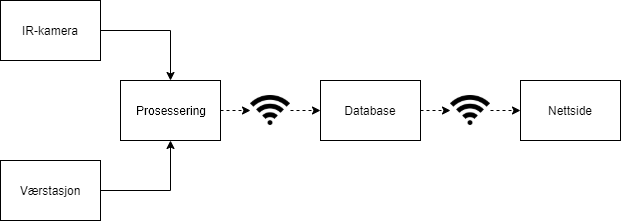
\includegraphics[width=0.9\textwidth]{design/designflytskjema.png}
    \caption{Blokkdiagram over systemet. Fuglene blir detektert av et infrarødt kamera og bildene prosesseres. Værdata samles inn. Dataen blir så sendt videre til en database og vist fram på en nettside.}
    \label{fig:blokkDig}
\end{figure}


\subsection{Kamera}\label{sec:design:kamera}

Et infrarødt kamera(heretter kalt IR-kamera) brukes til å detektere infrarød stråling. 
Infrarød stråling er elektromagnetisk stråling med en bølgelengde mellom $\SI{7}{\micro\meter}$ og $\SI{1}{\milli\meter}$ \cite{SNL-IR}. 
Alle objekter med en temperatur over det absolutt nullpunktet sender ut slik stråling, og bølgelengden og intensiteten til denne strålingen kan brukes for å avgjøre temperaturen til objektet. 
I dette designet brukes et IR-kamera for å detektere den infrarøde strålingen emittert fra fugler. 
Fugler er varmblodige og holder en kroppstemperatur på rundt $\SI{30}{\degree}$ \cite{snlfugl}.
De emittere infrarød stråling som i prinsippet kan detekteres av et infrarødt kamera, der himmelen bak vil emittere relativt mye mindre IR-stråling.

Et IR-kamera brukes i stedet for et vanlig kamera, da det gjør det enklere å detektere fuglene mot himmelen. 
Et godt eksempel på dette vil være når en hvit måke flyr foran hvite skyer. 
Farge til måken vil da kunne gå i ett med skyene, og gjør bildebehandlingen for å detektere fuglen svært vanskelig. 
Med et IR-kamera vil skyene emittere mindre infrarød stråling, og fuglen kan dermed detekteres. 
Videre vil et IR-kamera også gjøre det mulig å detektere fugler når det er mørkt, i motsetning til et konvensjonelt kamera. 
En ulempe med IR-kamera er at fuglenes fysiske trekk ikke er synlige, som for eksempel farge, som ville gjort det lettere å bestemme fuglenes art. 

\subsection{Deteksjon}\label{sec:design:deteksjon}

Prosesseringsenheten skal ta inn en kontinuerlig strøm av bilder fra kameraet og behandle denne bilde for bilde. 
Bildebehandlingen skal finne objekter i bildet, eller såkalte \textit{blobs}\footnote{Binary Large OBjects}. 
Objektene som skal oppdages er fugler, og disse vil skille seg ut fra bakgrunnen på grunn av deres høyere temperatur, som representeres ved at de har ulik farge fra bakgrunnen på bildene. 
Bildebehandlingen skal kunne detektere flere objekter i samme bilde. 
I tillegg skal den kunne se på forrige bilde for å finne ut om et objekt har beveget seg, og dermed kunne følge dette objektet gjennom en bildeserie. 
Slik unngås det at hver fugl telles en gang per bilde, men blir i stedet fulgt fra den kommer inn i synsvinkelen til kameraet til den går ut, og blir registrert som én fugl.

I utgangspunktet skal systemet detektere fugler i området foran vindturbinen, der det vil være stor sannsynlighet for at detekterte fugler vil kollidere med vindturbinen. Deteksjonsområdet ønskes å minimum dekke området som er vist i \autoref{fig:TurbinForan} og \ref{fig:TurbinSiden}. 
Videre plasseres kameraet slik at vindturbinen ikke er i synsvinkelen til kameraet, da dette vil kunne forstyrre målingene.


\begin{figure}[!htbp]%hentet fra https://www.cadblocksfree.com/en/wind-turbine.html
  \centering
  \begin{minipage}[b]{0.45\textwidth}
    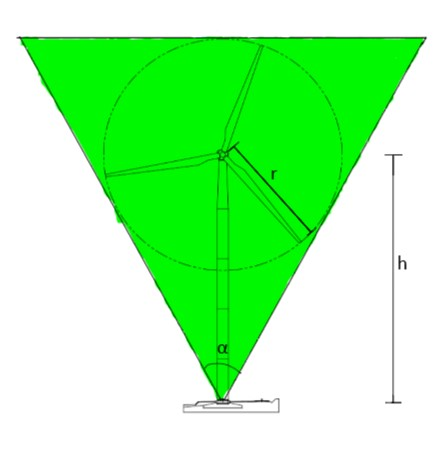
\includegraphics[width=\textwidth]{design/DeteksjonForan.jpg}
    \caption{Deteksjonsområdet til systemet sett fra framsiden til vindturbinen, markert i grønt. }
    \label{fig:TurbinForan}
  \end{minipage}
  \hfill
  \begin{minipage}[b]{0.45\textwidth}
    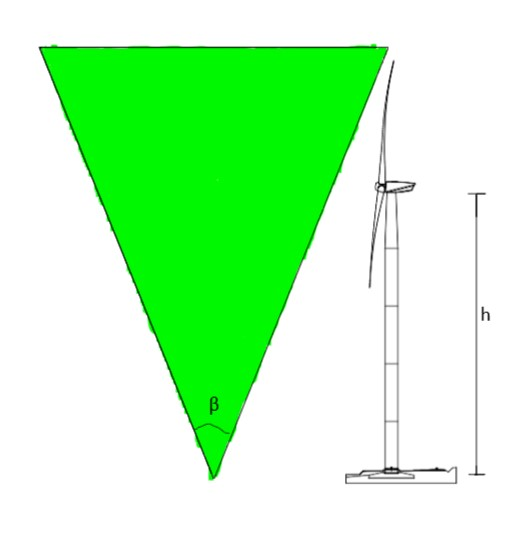
\includegraphics[width=\textwidth]{design/DeteksjonSiden.jpg}
    \caption{Deteksjonsområdet til systemet sett fra siden til vindturbinen, markert i grønt.}
    \label{fig:TurbinSiden}
  \end{minipage}
\end{figure}

Systemkrav \idref{id:areal} og \idref{id:rekkevidde} i \autoref{tab:systemkrav} er basert på vindturbinen Vestas v27-225kW \cite{vindturbin}.
Det er en vindturbin som står på Rye i Trondheim og dette området blir brukt som testarena.


\subsection{Værstasjon}\label{sec:design:vaerstasjon}
Systemet skal ha egne sensorer for innsamling av værdata. 
Dataene fra sensorene skal kunne knyttes opp mot fugleaktiviteten for å finne eventuelle sammenhenger i vær og fugleaktivitet. 
For eksempel, hvis all fugleaktivitet skjer når det ikke blåser, så vil kollisjon med vindturbiner være en mindre reell fare, siden turbinene ikke vil bevege seg i slikt vær. 

\subsection{Strukturelt}\label{sec:design:strukturelt}

Prosesseringsenheten og kameraet skal dele en boks. Boksen skal være festet til en påle for å heves over bakkenivå, slik at forstyrrelser eller skader fra dyr unngås, samt for å ikke tildekkes av snø eller vegetasjon. Videre skal boksen tilfredsstille systemkrav \idref{id:IPrating} om å være værbestandig, og dimensjonkravene \idref{id:størrelse} fra \autoref{tab:systemkrav}. Værsensorene skal være festet på samme påle som resten av systemet. Systemet henter strøm fra strømnettet.

\subsection{Database}\label{sec:design:database}

Det blir brukt en database for å lagre data fra værsensorene, kameraet og prosessoren. Det blir tatt utgangspunkt i at det er Wi-Fi dekning der produktet plasseres. Databasen vil brukes som et mellomledd mellom sensorene og nettsiden. Dermed trengs det ikke å skrive en protokoll for å overføre data. 


\subsection{Nettside}\label{sec:design:nettside}

Systemet vil ha en nettside som skal fremstille dataene som samles fra systemet. 
Måten dataen vises på skal være slik at den er lett forståelig og navigerbar for en bruker uten spesiell teknisk kompetanse. 
Dataen skal kunne sorteres etter behov for å se trender i fugleaktivitet, for eksempel time for time eller dag for dag. 
Det vil også være mulighet for eksportering av rådata direkte fra nettsiden. 

For at nettsiden ikke skal være veldig treg, må det være god kommunikasjon mellom nettside og database. 


\subsection{Systemkrav}\label{sec:design:systemkrav}

Tabell \ref{tab:systemkrav} viser systemkravene. 

\begin{table}[!htbp]
\centering
\caption{Systemkrav.}
\label{tab:systemkrav}
\resizebox{\textwidth}{!}{%
\begin{tabular}{|l|l|l|}
\hline
\multicolumn{3}{|l|}{Generelt}                                                                                                                              \\ \hline
\textbf{Kravnavn}           & \textbf{Beskrivelse}                                                                         & \textbf{id}                    \\ \hline
Mål                         & Systemet skal detektere og dokumentere fugleaktivitet i luften.                              & \idlabel{id:mål}               \\ \hline
Underlag                    & Området vil ha et flatt underlag.                                                            & \idlabel{id:underlag}          \\ \hline
Vegetasjon/miljø            & Området vil være minst 15x8m med åpent areal.                                                & \idlabel{id:areal}             \\ \hline
Toleranse/tetthet/IP-rating & Systemet skal være vanntett og tåle å stå ute i norske værforhold.                           & \idlabel{id:IPrating}          \\ \hline
Strømforsyning              & Systemet vil få strøm fra strømnettet.                                                       & \idlabel{id:strøm}             \\ \hline
Sensorer                    & Systemet vil ha temperatur, lufttrykk luftfuktighet, nedbørmåler og vindsensor.              & \idlabel{id:telemetri}         \\ \hline
\multicolumn{3}{|l|}{Deteksjon}                                                                                                                             \\ \hline
\textbf{Kravnavn}           & \textbf{Beskrivelse}                                                                         & \textbf{id}                    \\ \hline
Synsvinkel                  & Systemet vil bruke et infrarødt kamera med en minimum synsvinkel på $\ang{41}$x$\ang{31}$.   & \idlabel{id:kamera}            \\ \hline
Rekkevidde                  & Systemet skal ha en rekkevidde på minimum 50 meter.                                          & \idlabel{id:rekkevidde}        \\ \hline
Størrelse                   & Systemet skal minimum detektere fugler med størrelse ned til 300x100mm innenfor rekkevidden. & \idlabel{id:temperatur}        \\ \hline
\multicolumn{3}{|l|}{Fysiske dimensjoner}                                                                                                                   \\ \hline
\textbf{Kravnavn}           & \textbf{Beskrivelse}                                                                         & \textbf{id}                    \\ \hline
Dimensjoner                 & Produktet vil være mindre enn 200x300x300mm ekskudert stativ.                                & \idlabel{id:størrelse}         \\ \hline
\multicolumn{3}{|l|}{Overføring, behandling og fremstilling av data}                                                                                        \\ \hline
\textbf{Kravnavn}           & \textbf{Beskrivelse}                                                                         & \textbf{id}                    \\ \hline
Prosesseringsenhet          & Dataene vil behandles av en liten ettkortsdatamaskin.                                        & \idlabel{id:prosessor}         \\ \hline
Programvare                 & Programvaren vil være basert på åpen kildekode.                                              & \idlabel{id:opensource}        \\ \hline
Treffrate                   & Programvaren skal være god nok til å gi en treffrate  $\geq$75\%.                            & \idlabel{id:treffrate}         \\ \hline
Overføring internt          & Systemet vil bruke USB til å overføre data mellom kamera og prosesseringsenhet.              & \idlabel{id:internoverføring}  \\ \hline
Overføring eksternt         & Systemet vil bruke Wi-Fi for å overføre data fra prosesseringsenhet og databasen.            & \idlabel{id:eksternoverføring} \\ \hline
Fremstilling av data        & Resultatene vil fremstilles på en nettside.                                                  & \idlabel{id:nettside}          \\ \hline
\end{tabular}
}
\end{table}


